\section{Algorithm Details}
\label{section:algorithmoverview}
In this section we explain how HashFlow works in detail, and present some theoretical analysis results, 
which are based on a probabilistic model.

\subsection{Data Structures and Algorithm}
The data structure of HashFlow is composed of a main table (${\mathbf M}$) and an ancillary table (${\mathbf A}$), 
each being an array of buckets, and each bucket (also called as cell) can store a flow record
in the form of \emph{(key, count)}, as mentioned in Section~\ref{section:background}. 
In the main table ${\mathbf M}$, flow ID will be used as \emph{key}, 
while in the ancillary table ${\mathbf A}$, a digest of flow ID will be used as \emph{key} to save the memory space.
We have a set of $d+1$ independent hash functions, i.e., $h_1, h_2, \cdots, h_d$, and $g$, 
where $d$ is a positive integer (we  call $d$ the  \emph{depth} of ${\mathbf M}$, and typically $d=3$). 
Each hash function $h_{i} (1 \le i \le d)$  randomly maps a flow ID to one bucket in ${\mathbf M}$, 
while $g$ maps the ID to one bucket in ${\mathbf A}$. 
A digest can be generated from the hashing result of the flow ID with any $h_i$.
When a packet arrives, HashFlow updates ${\mathbf M}$ and ${\mathbf A}$ with the following 
two strategies, as shown in Algorithm \ref{alg: process_packet}.

1) \textbf{Collision Resolution.} When a packet $p$ arrives, we first map it into the bucket indexed 
at $idx=h_1(p.\text{flow\_id})$ in the main table ${\mathbf M}$.  
If ${\mathbf M}[idx]$ is empty, we just put the flow ID and a count of 1 in the bucket (line 5$\sim$ 6).
If the bucket is already occupied by packets of this flow earlier, 
we just simply increment the count by 1 (line 7 $\sim$ 8). 
In either case, we have found a proper bucket for the packet, and the process finishes. 
If neither of the two cases happen, then a collision occurs, 
and we repeat the same process but with $h_2, h_3, \cdots, h_d$ one by one, 
until a proper bucket is found for the packet. 
This is a simple collision resolution procedure. 
Unlike HashPipe and ElasticSketch, it does not evict existing flow record from the main table, 
thus prevents a record from being split into multiple records. 

If collision cannot be resolved in the main table, 
then we try to record it in the ancillary table ${\mathbf A}$.
Here the action is more intrusive, 
as an existing flow will be replaced (discarded) if it collides with the new arrival (line 16 $\sim$ 19).

2) \textbf{Record Promotion.} If, in the ancillary table ${\mathbf A}$, $p$ succeeds to find the right bucket to reside, 
then it updates the packet count field of the record. 
Moreover, if the corresponding flow record keeps growing and the packet count becomes large enough, 
then we will promote the record by re-inserting it into the main table,
thus prevents large flows from being discarded. 
To implement this strategy, we keep in mind the sentinel flow record that has the smallest packet count 
among those records that collide with $p$ in the collision resolution procedure (line 9 $\sim$ 11). 
When a flow record in the ancillary table should be promoted, it will replace this sentinel  
we have kept in mind (line 22 $\sim$ 23).
We note that, instead of the flow ID, a shorter digest is used as keys in the ancillary table to 
reduce memory consumption. This may mix flows up, but with a small chance. When doing record promotion, we simply extract the flow ID from the current packet.


 
\begin{algorithm}[ht!]
    \caption{Update Algorithm of HashFlow on arrival of $p$}
    \label{alg: process_packet}
    \algrenewcommand\algorithmicwhile{\textbf{when}}
    \begin{algorithmic}[1]
        \State{//Collision Resolution}
        \State{$flowID \gets p.\text{flow\_id}, min \gets \infty, pos \gets -1$}
        \For{$i=1$ to $d$}
        \State{$idx\gets h_{i}(flowID)$}
        \If{${\mathbf M}[idx].key==NULL$}
        \State{${\mathbf M}[idx] \gets (flowID, 1)$}
        \Return
        \ElsIf {${\mathbf M}[idx].key == flowID$}
        \State{Increment ${\mathbf M}[idx].count$ by 1}
        \Return
        \ElsIf{${\mathbf M}[idx].count < min$}
        \State{$min \gets {\mathbf M}[idx].count$}
        \State{$pos \gets idx$}
        \EndIf
        \EndFor
        \State{$idx\gets g(flowID)$}
        \State{$digest \gets h_{1}(flowID)\%(2^{\text{digest width}})$}
        \If{${\mathbf A}[idx].count==0$ or ${\mathbf A}[idx].key \neq digest$}
        \State{${\mathbf A}[idx] \gets (digest, 1)$}
        \ElsIf{${\mathbf A}[idx].count < min$}
        \State{Increment ${\mathbf A}[idx].count$ by 1}
        \Else
        \State{//Record Promotion}
        \State{${\mathbf M}[pos].key \gets flowID$}
        \State{${\mathbf M}[pos].count \gets {\mathbf A}[idx].count+1$}
        \EndIf
    \end{algorithmic}
\end{algorithm}


We use a simple example with $d=2$ to illustrate the algorithm, as depicted in Fig. \ref{fig:datastructure}.
When a packet of flow $f_1$ arrives, $h_1$ maps it into an empty bucket indexed at $h_1(f_1)$, 
so the record becomes $(f_{1}, 1)$. 
When a packet of flow $f_2$ arrives, $h_1$ maps it into a bucket indexed at $h_1(f_2)$, 
where the record $(f_{2}, 5)$ has the same key, 
and the counter is simply incremented. 
When a  packet of flow $f_3$ arrives, it collides with the record $(f_4, 4)$ in the bucket indexed at $h_1(f_3)$. 
Then we try to resolve collision with $h_2$, but again, 
the packet collides with the record $(f_5, 10)$ in the bucket at $h_2(f_3)$. 
So we have to use $g$ to find a place in the ancillary table for the packet. 
Sadly, it collides again with the record $(f_6, 8)$, and we let it replace the existing one.
The last packet is from  flow $f_{7}$, and it goes through a similar process to that of $f_3$. 
The difference is that, at last, this packet finds its corresponding flow record of $(f_7,7)$ in the ancillary table, and after being updated the record appears to have greater packet count (i.e., 8) than the sentinel flow which has the packet count of 7. 
So we promote $(f_7, 8)$ by inserting it back into the main table, evicting the sentinel one. 
 


\begin{figure}
    \centering
    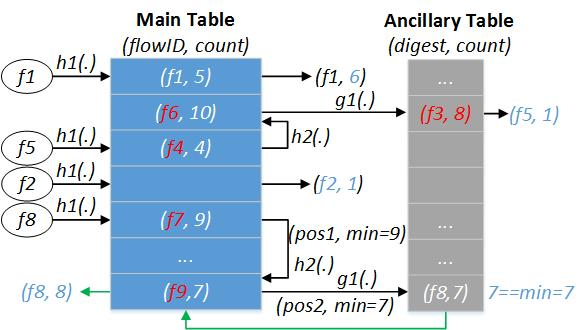
\includegraphics[width=\linewidth]{./figures/datastructure/datastructure}
    \caption{An example of HashFlow}
    \label{fig:datastructure}
\end{figure}


In Algorithm \ref{alg: process_packet}, we use multiple independent hash functions $h_i$$(i=1,2,\cdots,d)$ in a single main table ${\mathbf M}$.
Another choice is to use multiple small hash tables ${\mathbf M}_{i}$, each of which corresponds to an independent  hash function $h_{i}$. 
Algorithm \ref{alg: process_packet} can be modified straightforwardly: 
update the $i$-th small table ${\mathbf M}_{i}$ instead of ${\mathbf M}$ (line 5 $\sim$ 12),
remember which small table the sentinel record resides in (line 10 $\sim$ 11), 
and evict the sentinel record in the right small table (line 22 $\sim$ 23) to do record promotion.
In addition, we introduce a weight $\alpha (0<\alpha<1)$, 
such that the number of buckets in $\mathbf{M}_{i+1}$ is $\alpha$ times that in $\mathbf{M}_i$.

Readers may notice that HashPipe uses a similar scheme of pipelined tables, 
but there are a few important differences. 
First, HashFlow uses pipelined tables together with an ancillary table.
Second, the update strategy of these pipelined tables is different from that of HashPipe. 
Third,  our collision resolution procedure on the main table can be analyzed theoretically, 
based on which we can achieve a concrete performance guarantee on the number of accurate 
flow records that HashFlow can maintain.

\subsection{Analysis}
\label{analysis}
In the section, we propose a probabilistic framework that models the utilization of the  main table.
We first analyze the case where a multi-hash table is used for the main table,
then the case where pipelined tables are used. 
In either case, we assume that there are $m$ distinct flows fed into the main table, 
which has $n$ buckets in total, and uses $d$ hash functions.


%In the section we will analyze the utilization of a Main Table in the form of a normal hash table as well as a hierarchical hash table. Suppose the depth of a hash table is $d$, i.e., there are $d$ hash functions associated with it. It consists of $n$ cells and there are $m$ distinct flows feed into it. The \emph{utilization} is defined as $utilization=\frac{n'}{n}$, where $n'$ is the number of flows cached successfully. 

\textbf{Multi-hash table.} First, consider the case when $d=1$, 
where the analysis follows a classic ball and urn problem\cite{urn}.
After inserting $m_1=m$ flows randomly into $n$ buckets, 
the probability that a given bucket is empty is 
\[\label{equation1}
p_1 = (1 - \frac{1}{n})^{m_1} \approx e^{-\frac{m_1}{n}},
\]
and the utilization of the table is 
$u_{1}=1-p_{1}= 1 - e^{-\frac{m_1}{n}}.$
Since each bucket can contain only one flow record due to our collision resolution strategy, 
the number of flows that fail to be cached in $\mathbf{M}$ after this round is $m_1-n\times(1-p_1)$.

Now consider the case of $d=2$. 
Essentially, a flow tries another bucket with $h_2$ if it finds out 
that the first bucket it tries has already been occupied. 
Since we don't care which exact flow is stored in the table, 
we slightly change the update process to the following one.
We take two rounds. In the first round, 
we feed all the $m_1$ flows into the table with $h_1$, exactly the same as $d=1$.
In the second round, we feed all the remaining flows that have not been kept in $\mathbf{M}$ into the table again, 
but this time with $h_2$. 
Assume $\mathbf{M}$ is empty before the second round starts, 
then after the $m_2=m_1-n\times(1-p_1)$ flows left by the first round have been inserted in the second round, 
a bucket will be empty with probability $e^{-\frac{m_2}{n}}$. 
However, $\mathbf{M}$ is actually not empty before the second round, 
and at that time a bucket in it is empty with probability $p_1$.
Since $h_1$ and $h_2$ are independent, we know after the second round, 
the probability that a bucket is still empty becomes $p_2 \approx p_1 \times e^{-\frac{m_2}{n}}$, 
and the number of flows that have not been inserted into $\mathbf{M}$ will be $m_3=m_1-n\times(1-p_2)$.
The utilization of $\mathbf{M}$ now becomes $u_2=1-p_2$.

The analysis for the slightly changed process can be extended to cases when $d>2$. 
In the $k$-th round, $m_k$ flows are fed into a hash table with a new hash function $h_k$, 
where there are already $n \times (1-p_{k-1})$ buckets being occupied in the previous rounds. 
Then after the $k$-th round, the probability that a bucket is empty is
\begin{eqnarray}
\label{xx1}
p_k & \approx &p_{k-1} \times e^{-\frac{m_k}{n}} \nonumber \\
& = & p_{k-1} \times e^{-\frac{m_1-n \times (1-p_{k-1})}{n}} \nonumber \\
& = & p_{k-1} \times e^{1-\frac{m_1}{n}-p_{k-1}} \nonumber \\
& = & p_{k-1} \times e^{1-\frac{m}{n}-p_{k-1}}
\end{eqnarray}
for $k \ge 2$. With Equation (\ref{xx1}), for any given $d$, $m$, and $n$, 
we can recursively compute the probability $p_d$ that a bucket is empty in the hash table after $d$ rounds. 
Then the utilization of the hash table will be $1-p_d$. 
We note that there is a slight difference between this model and our multi-hash table, as will be shown later.

\iffalse
In the case of $d=k, k\ge 2$, suppose the probability that a given cell is empty after the first $k-1$ runs of insertion is $p_{k-1}$. The number of flows that are waiting to be cached using the $k^{th}$ hash function is $m - n(1-p_{k-1})$, so the probability that there is no flow mapped to a given cell during this run of insertion is
\begin{equation}\label{equation3}
(1 - \frac{1}{n})^{m - n(1- p_{k-1})}\approx (\frac{1}{e})^{p_{k-1}}\cdot(\frac{1}{e})^{(\frac{m}{n} - 1)}
\end{equation}

And the probability that a cell is empty after $k$ runs of insertion is :
\begin{equation}\label{equation4}
p_k = p_{k-1}\cdot (\frac{1}{e})^{p_{k-1}}\cdot(\frac{1}{e})^{(\frac{m}{n} - 1)}
\end{equation}
and the utilization of the hash table is:
\begin{equation}\label{equation5}
u_k = \frac{n - n\times p_k}{n} = 1 - p_k
\end{equation}
\fi



\begin{figure*}[t]
    \centering
    \mbox{
        \subfigure[Multi-hash Table\label{multihash}]{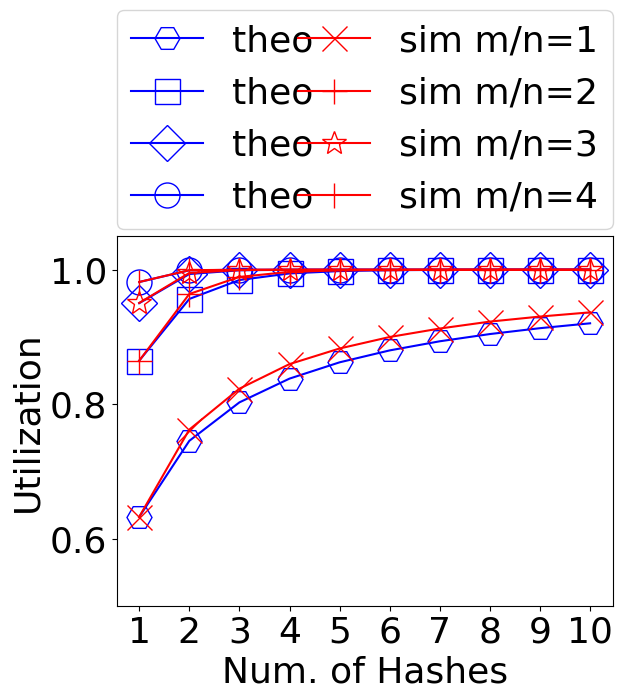
\includegraphics[width=0.24\linewidth]{figures/exp84481/hash_table_utilization}}
        \subfigure[Pipelined Tables\label{pipeline1}]{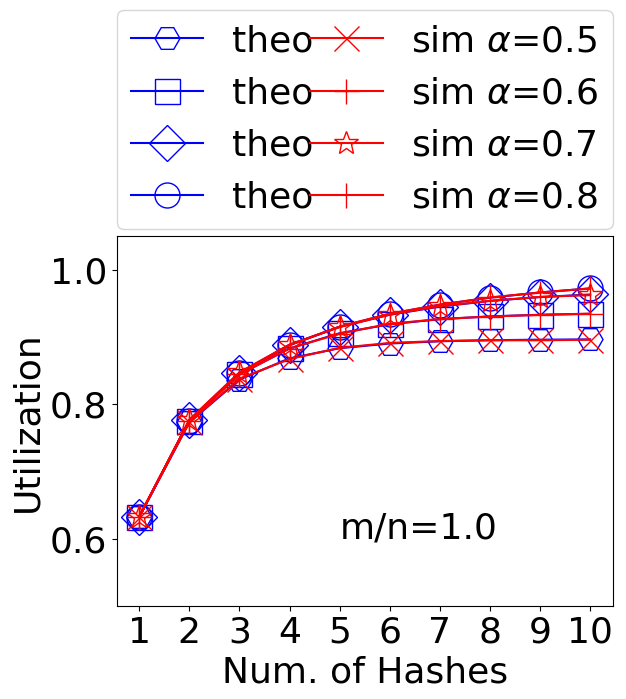
\includegraphics[width=0.24\linewidth]{figures/exp84489/pipelined_tables_utilization_ratio_10}}
        \subfigure[Pipelined Tables\label{pipeline2}]{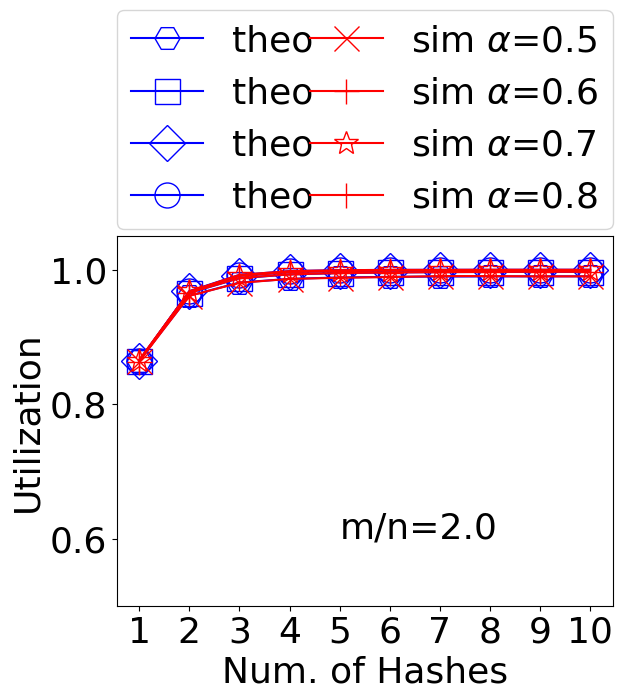
\includegraphics[width=0.24\linewidth]{figures/exp84489/pipelined_tables_utilization_ratio_20}}
        \subfigure[Improvement on Utilization\label{improvement}]{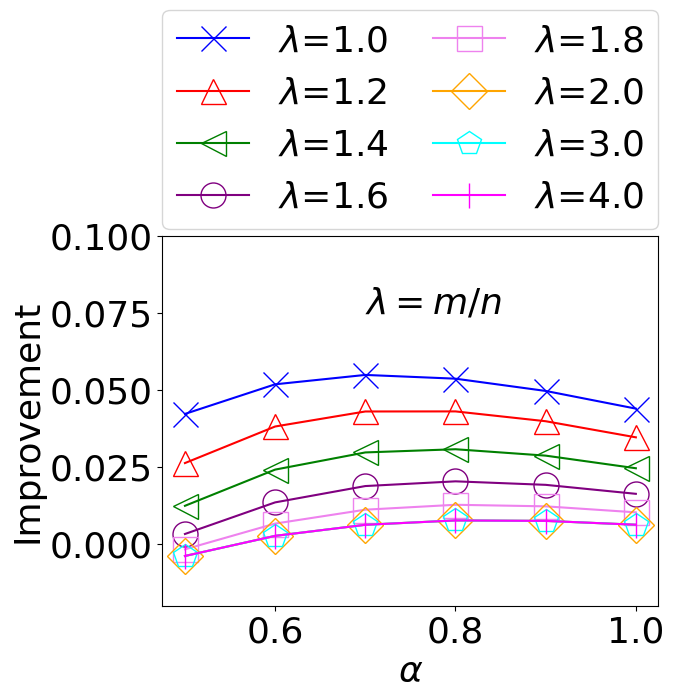
\includegraphics[width=0.24\linewidth]{figures/exp84488/improvement}}
    }
    \caption{Utilization of the multi-hash table and the pipelined tables}
    \label{fig:pipelinedtablesutilizationratio}
\end{figure*}

\textbf{Pipelined tables.}
Let $n_k$ be the number of buckets in the $k$-th table $\mathbf{M}_k$ such that $n_{k+1}=\alpha \times n_k$, 
where $\alpha$ is the  pipeline weight.
We perform a similar modification to our collision resolution procedure with pipelined tables, 
such that in the $k$-th round, 
all packets goes though the $k$-th table before they are fed into the $k+1$-th table in the $k+1$-th round.
We use the same notations $p_k$, $m_k$ and $u_k$ as those in the first model.
Since $\sum_{k=1}^dn_k=\sum_{k=1}^d(\alpha^{k-1} \times n_1)=\frac{1-\alpha^{d}}{1-\alpha} \times n_1$, 
we get $n_1=\frac{1-\alpha}{1-\alpha^{d}} \times n$, 
and $n_k=\alpha^{k-1} \times \frac{1-\alpha}{1-\alpha^{d}} \times n$.

The first round works exactly the same as that in the previous model, 
so we get $p_{1}=(1 - \frac{1}{n_1})^{m_1} \approx e^{-\frac{m_1}{n_{1}}}$, 
$u_1=1-p_1$, and $m_2=m_1-n_{1}\times(1-p_1)$.

For the $k$-th round, we know $m_k$ flows are to be fed into the table $\mathbf{M}_{k}$ with $n_k$ buckets, 
so we get $p_{k} \approx e^{-\frac{m_k}{n_{k}}}$, 
and the number of flows left after this round is 
\begin{equation}
\label{xxx1}
m_{k+1}  =  m_{k}-n_{k}\times(1-p_k). 
\end{equation}
Dividing  both sides of Equation (\ref{xxx1}) by $n_{k+1}$, we get 
\begin{eqnarray}
\frac{m_{k+1}}{n_{k+1}} & = & \frac{n_k}{n_{k+1}}  \times \frac{m_{k}-n_{k}\times(1-p_k)}{n_k} \nonumber \\
& = & \alpha^{-1} \times \left( \frac{m_k}{n_k} - 1 + p_k  \right), \nonumber
\end{eqnarray}
which is just
\begin{equation}
\label{xxx2}
-\ln p_{k+1}=\alpha^{-1} \times (-\ln p_k -1 + p_k).
\end{equation}

From Equation (\ref{xxx2}), we finally get 
\begin{equation}
\label{xxx3}
p_{k+1}=(p_k)^{\frac{1}{\alpha}} \times e^{\frac{1-p_k}{\alpha}}. 
\end{equation}

With Equation (\ref{xxx3}), for any given $d$, $m$, and $n$, 
we can recursively compute the probability $p_k (1 \le k \le d)$ that a bucket is empty in the $k$-th hash table.
Then the utilization of the pipelined tables will be 
\begin{equation}
\label{pipelineutil}
\frac{\sum_{k=1}^{d} (n_k \times (1-p_k))}{\sum_{k=1}^{d} n_k} = 1- \frac{1-\alpha}{1-\alpha^{d}} \times \sum_{k=1}^{d}(\alpha^{k-1} \times p_{k}).
\end{equation}

\iffalse
$m_i$ is the number of flows that arrives at this table. Thus we have
\begin{IEEEeqnarray}{crc} 
n = \sum_{i =1}^d n_i = \sum_{i =1}^d \alpha^{i-1}n_1\\
m = m_1
\end{IEEEeqnarray}

We denote $\sum_{i =1}^d \alpha^{i-1}$ by $\delta$. For the first table, after inserting $m_1 = m$ flows, the probability that a given cell is empty is
\begin{IEEEeqnarray*}{crc}
    p_1 = (1 - \frac{1}{n_1})^{m_1}\approx (\frac{1}{e})^{\frac{m_1}{n_1}} = (\frac{1}{e})^{\delta\cdot\frac{m}{n}}
\end{IEEEeqnarray*}

For the $k^{th}$ table ($k= 2, \cdots, d$), after inserting $m_k$ flows, the probability that a given cell is empty is 
\begin{equation}
p_k = (1 - \frac{1}{n_k})^{m_k} \approx (\frac{1}{e})^{\frac{m_k}{n_k}}
\end{equation}

Notice $m_k = m_{k - 1} - n_{k - 1}(1 - p_{k - 1})$, we get
\begin{IEEEeqnarray*}{crc}
    \frac{m_k}{n_k} &=& \frac{m_{k - 1} - n_{k - 1}(1 - p_{k - 1})}{\alpha\cdot n_{k-1}} \\
    &=& \frac{1}{\alpha}(p_{k - 1} - \ln p_{k - 1} - 1)
\end{IEEEeqnarray*}

So $p_k$ corresponding to each sub-table can be given by
\begin{IEEEeqnarray*}{crc}
    p_k = e^{\frac{1}{\alpha}(1-p_{k-1})}(p_{k-1})^{\frac{1}{\alpha}}
\end{IEEEeqnarray*}

The utilization of the tables is 
\begin{IEEEeqnarray*}{crc}
    utilization &=& 1  - \frac{1}{n}\sum_{i = 1}^{d}n_kp_k
    = 1 - \frac{1}{\delta}\sum_{i = 1}^{d}\alpha^{i - 1}p_i
\end{IEEEeqnarray*}
\fi

Now we will show how accurate the models are. 
In Fig. \ref{multihash},
we compare the utilization provided by our multi-hash table model against the results from simulations on some real traces.
We use $n=$100K buckets, with different depth $d$ from 1 to 10, 
and vary the traffic load $m/n$ from 1 to 4. As can be seen there, 
only under a light load of $m/n=1$, there is a slight difference between the model and the real algorithm.
When $m/n \ge 2$, the multi-hash table model provides nearly perfect predictions.

Fig. \ref{pipeline1} and Fig. \ref{pipeline2} depict the utilization provided by our model on pipelined tables, 
as well as results from simulations, for traffic load $m/n=1.0$ and 2.0, respectively. 
We use a similar setting as above, with $n=$100K and $d$ from 1 to 10,
but we vary the pipeline weigh $\alpha$ between 0.5 to 0.8. 
This time the model and the simulation results match  quite well, 
since  arranging the packet arrivals in rounds, as we have done in the model,  
actually does not affect the final probability (we omit the proof due to space limitations).

With these two models, we can compute the utilization of our main table, 
as long as the traffic load $m/n$ is known. Since each record is accurate 
(neglecting the minor chance that a flow record promoted back to the main 
table happens to have an inaccurate count), this provides a concrete prediction 
on the number of records HashFlow can report. 
We can see that more hash functions will improve the utilization.
For example, in the case of $m/n=1$, the utilization  increases from 63\% to 80\% 
when $d$ is increased from 1 to 3, and from 83 to 92 when $d$ is increased from 3 to 10.
As more hash functions require more hash operations and memory accesses in the worst case, 3 hash functions seems to be a  sweet spot, and we use $d=3$ by default in our evaluations.

Fig. \ref{improvement} shows, when $d=3$, 
pipelined tables always improves the utilization upon  multi-hash table, regardless of the traffic load.
As shown there, when $\alpha=0.7$ and $m/n=1$, up to 5.5\% more utilization can be achieved.
Our evaluation will adopt the pipelined scheme, where $\alpha=0.7$ seems to be the best choice.

%. For example, $H$ is a hash table with 100K cells and there are 3 hash functions, i.e., $h_1$, $h_2$ and $h_3$, associated with it. The hash functions can map a flow ID to the hash table independently and randomly. We refer to this hash table as \emph{normal} hash table. We reconstruct the hash table such that the hash table consists of 3 sub-tables and $h_1$, $h_2$ and $h_3$ are associated with the sub-tables respectively. The sizes of the sub-tables are determined by a  \emph{hierarchy coefficient} $\alpha$ ($0 < \alpha <= 1$) such that $S_i = \alpha\times S_{i-1}$ for $i = 2, 3$ where $S_i (i = 1, 2, 3)$ is the size of sub-table $i$. We feed 100K randomly generated flow IDs into the normal hash table as well as hierarchical hash tables with various $\alpha$ and then calculate the utilization of the hash tables. Fig.~\ref{fig:simulator_hierarchical_hashtable_performance} shows that the utilization of hierarchical hash tables are better than that of a normal hash table when the value of $\alpha$ is no less than 0.5. Since the MT of HashFlow is a hash table essentially, the utilization of MT should be higher if it is organized hierarchically and the hierarchy coefficient is set properly. 
%\begin{figure}
%    \centering
%    \begin{minipage}{0.24\textwidth}
%    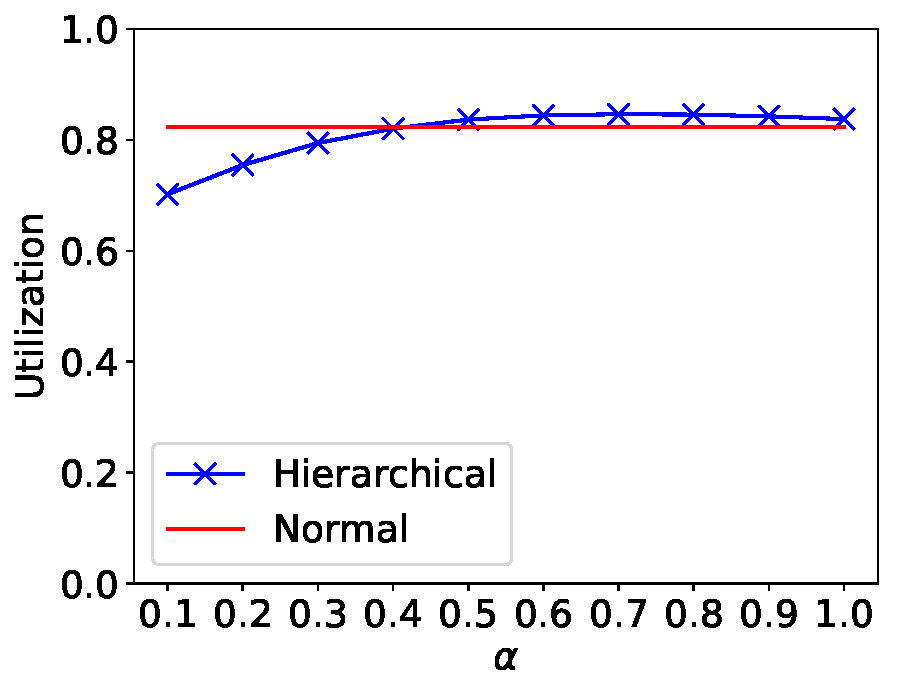
\includegraphics[width=\linewidth]{figures/exp84483/hash_table_utilization}
%    \caption{The utilization of a normal hash table as well as that of a hierarchical hash table as the value of $\alpha$ increases from 0.1 to 1.0.}
%    \label{fig:simulator_hierarchical_hashtable_performance}
%    \end{minipage}
%\end{figure}

